\chapter{Sprint1}
\section{Introduction}
In this chapter, we will design and implement the functionalities of Sprint 1 of our project.
We will first present the sprint backlog, where we will detail the requested features. The next step is to analyze the specified functionalities. Finally, we will show the output of this sprint.
\section {Backlog Sprint}
\begin{table}[h]
\centering

\begin{tabular}{|c|p{5cm}|c|p{10cm}|}
\hline
ID & US & Estimation & Tâches à réaliser \\
\hline
 & & & \begin{tabular}[c]{@{}l@{}}
 - Setting up the work environment
    \\- Preparing the project structure Backend
    \\- Preparing the libraries and creating the REST APIs
    \\ - Preparing the database \end{tabular} \\
\hline
1 & as a collaborator, I want to authenticate to the platform & 3 &\begin{tabular}[c]{@{}l@{}}- Creation of the graphical interface (UX) for authentication for \\ an Orange collaborator Administrator/Coordinator/Exepert\\

-Implement the interface
\\-Implement the necessary methods to ensure user authentication
\\-Test \end{tabular}\\
\hline
2 & as a collaborator, I want to logout of the platform & 2 & \begin{tabular}[c]{@{}l@{}} Creation of the graphical interface (UX) for logout for \\an Orange collaborator Administrator/Coordinator/Exepert\\

    -Implement the interface
    \\-Implement the necessary methods to ensure user logout
    \\-Test \end{tabular}\\
\hline
3 & As a collaborator, I want to update my profile &2 & \begin{tabular}[c]{@{}l@{}}- Creation of the graphical interface (UX) for updating profile \\
    - Implement the interface \\
    - Implement the necessary methods to update profile details \\
    - Test \end{tabular} \\
\hline
4 & As an ODC collaborator, I want to change my password &1& \begin{tabular}[c]{@{}l@{}}- Creation of the graphical interface (UX) for changing password \\
    - Implement the interface \\
    - Implement the necessary methods to change password \\
    - Test \end{tabular} \\
    \hline     
\end{tabular}

\end{table}
\newpage 
\begin{table}[h]
    \centering
    \begin{tabular}{|c|p{5cm}|c|p{10cm}|}
        \hline
        ID & US & Estimation & Tâches à réaliser \\
        \hline
        5 & As a super admin, I want to add an ODC coordinator & 2& \begin{tabular}[c]{@{}l@{}}- Creation of the graphical interface (UX) for adding an ODC\\ coordinator \\
            - Implement the interface \\
            - Implement the necessary methods to add an ODC coordinator \\
            - Test \end{tabular} \\
            \hline
    6 &\begin{tabular}[c]{@{}l@{}} As a super admin,\\ I want to enable/disable \\an ODC collaborator \\coordinator/Expert \end{tabular} & 3& \begin{tabular}[c]{@{}l@{}}- Creation of the graphical interface (UX) for enabling/disabling an \\ODC collaborator coordinator/Expert \\
        - Implement the interface \\
        - Implement the necessary methods to enable/disable an ODC \\collaborator coordinator/Expert \\
        - Test \end{tabular} \\
        \hline
        7 &  As a super admin,I want to view ODC Coordinators/Experts list & 3& \begin{tabular}[c]{@{}l@{}}- Creation of the graphical interface (UX) for viewing \\ODC coordinator/experts list \\
            - Implement the interface \\
            - Implement the necessary methods to view ODC experts list \\
            - Test \end{tabular} \\
            \hline
        7 & As an ODC Coordinator, I want to add an ODC Expert &2& \begin{tabular}[c]{@{}l@{}}- Creation of the graphical interface (UX) for adding an\\ ODC Expert \\
            - Implement the interface \\
            - Implement the necessary methods to add an ODC Expert \\
            - Test \end{tabular} \\
            \hline        
            8 & As an ODC Coordinator, I want to enable/disable an ODC Expert &2 & \begin{tabular}[c]{@{}l@{}}- Creation of the graphical interface (UX) for enabling\\/disabling an ODC Expert \\
                - Implement the interface \\
                - Implement the necessary methods to enable/disable \\an ODC Expert \\
                - Test \end{tabular} \\
                \hline
                9 & As an ODC Coordinator,I want to view ODC experts list &2 & \begin{tabular}[c]{@{}l@{}}- Creation of the graphical interface (UX) for viewing \\ODC experts list \\
                    - Implement the interface \\
                    - Implement the necessary methods to view ODC experts list \\
                    - Test \end{tabular} \\
                    \hline
                
    \end{tabular}
    \caption{Backlog for the First Sprint}
\label{tab:Backlog for the First Sprint}
\end{table}
\newpage
\section{Use Case Diagram for Sprint 1} 
The following figure represents the use case diagram for our first sprint.
\begin{figure}[h!]
    \centering
    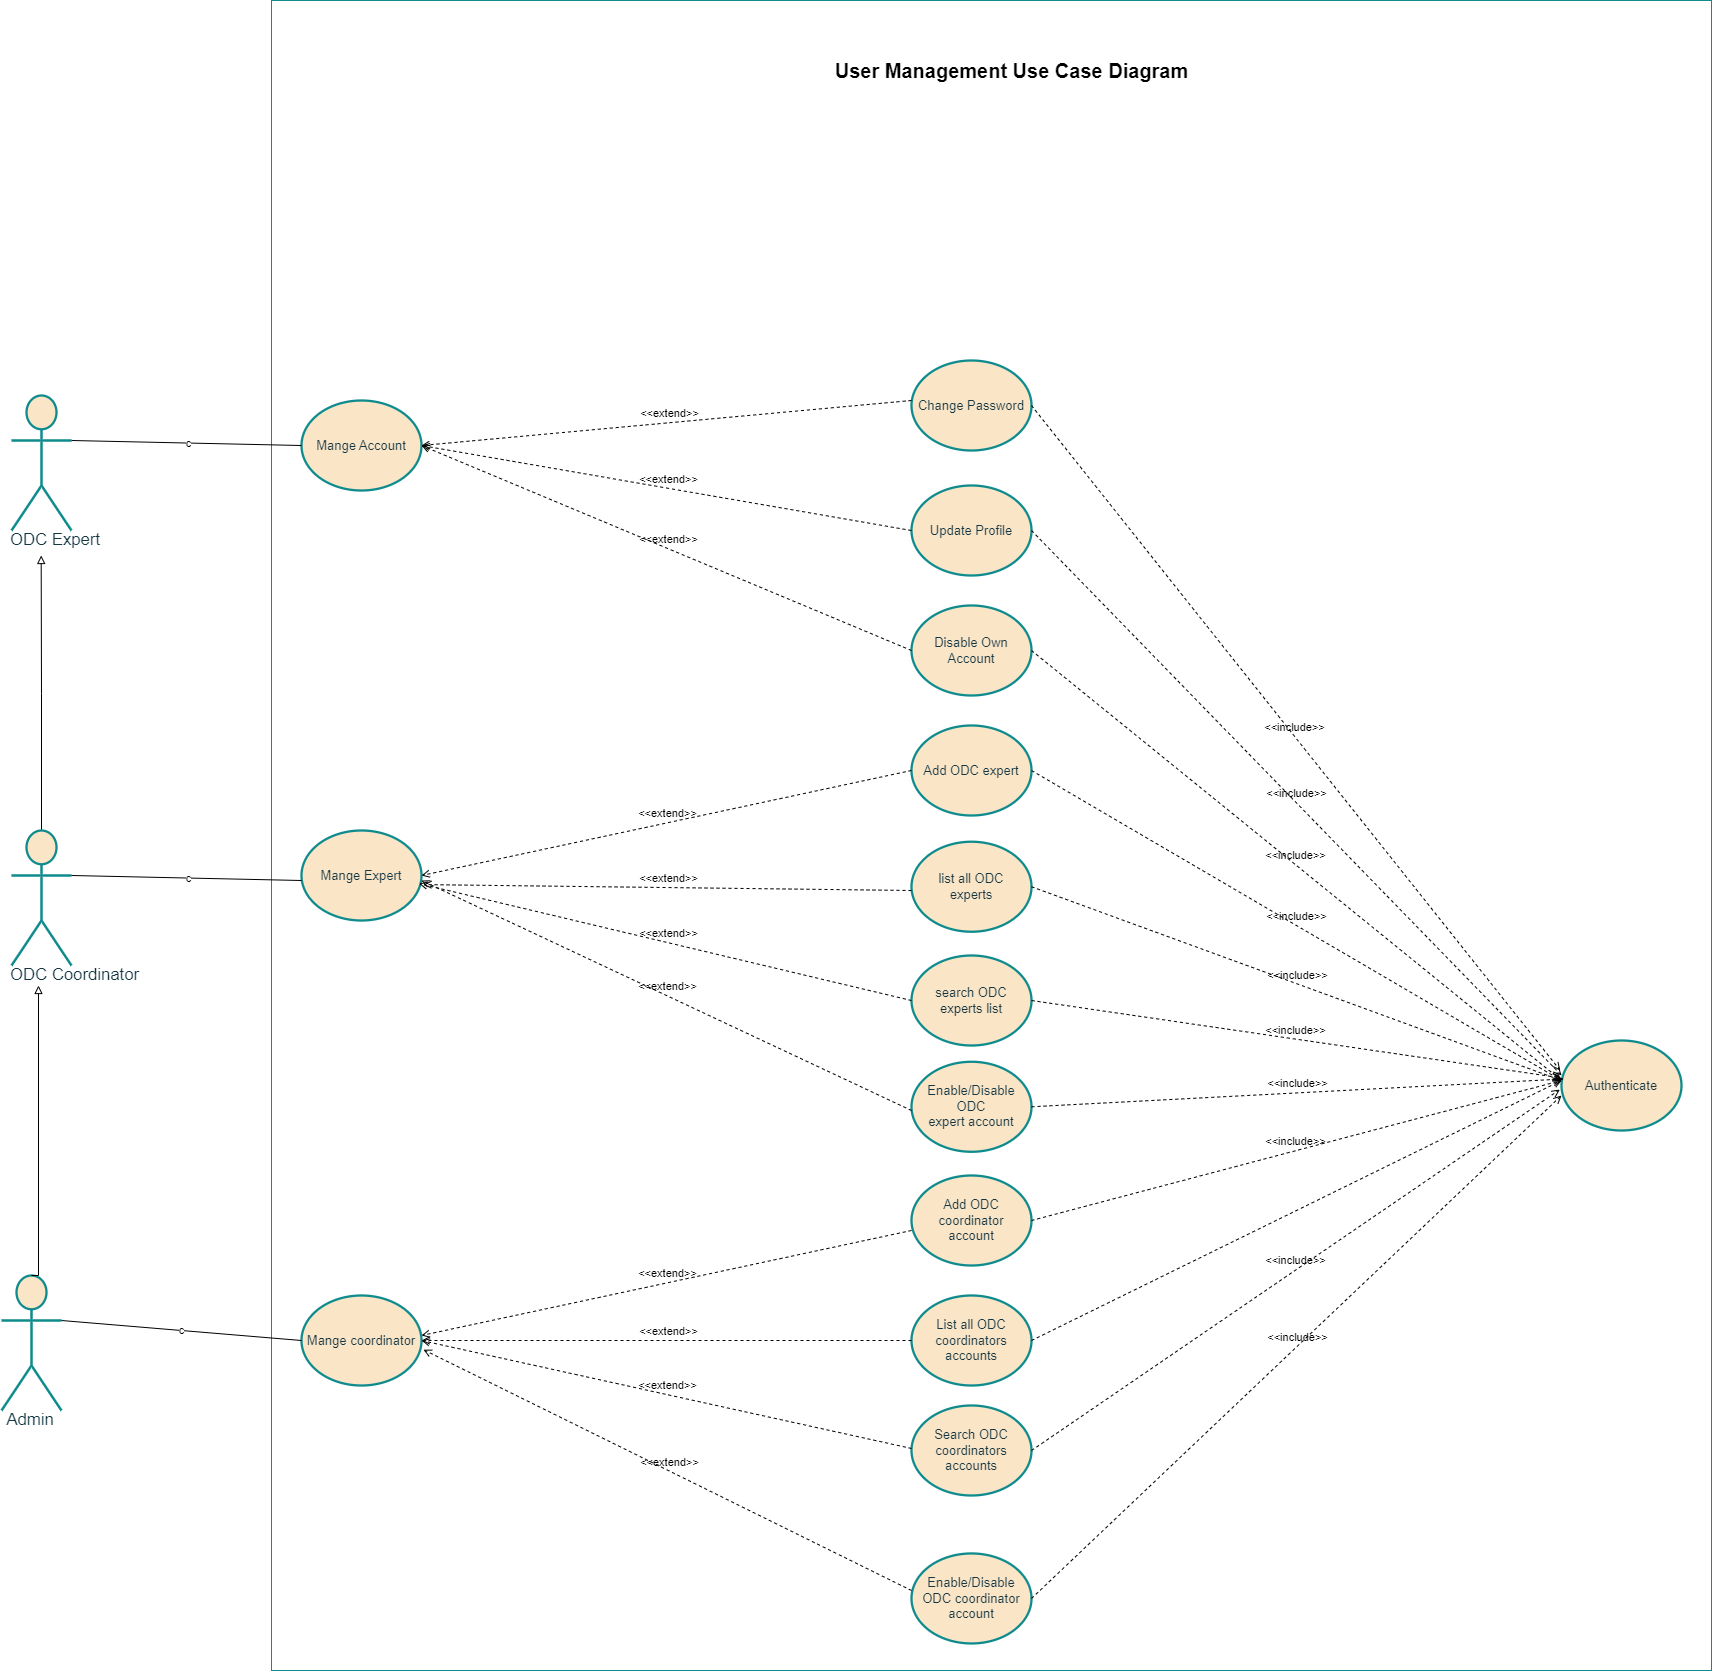
\includegraphics[height=1\textwidth]{images/usecaseS1.png}
    \caption{Use Case Diagram for Sprint 1}
    \label{fig:Use Case Diagram for Sprint 1}
\end{figure}
\newpage 

\subsection{Textual Description of the Use Case "Authenticate"}
\begin{table}[h]
    \centering
    \begin{tabular}{|c|c|}
        \hline
        Use Case & authenticate \\
        \hline
    Actor &\begin{tabular}[c]{@{}l@{}} User: Collaborator/Administrator


    \end{tabular} \\
        \hline
        Brief Description &\begin{tabular}[c]{@{}l@{}} The user must be registered in the database and must know their credentials
        \end{tabular} \\
            \hline
            Pre-condition &\begin{tabular}[c]{@{}l@{}} The user must have their access parameters
            \end{tabular} \\
                \hline
                Post-condition &\begin{tabular}[c]{@{}l@{}} The user is successfully authenticated
                \end{tabular} \\
                    \hline
                    Main Scenario &\begin{tabular}[c]{@{}l@{}} 1. The user enters their credentials (email and password) in the appropriate fields \\and submits the form.
                       \\ 2. The system verifies the information entered by the user
                        \\3. The system displays the appropriate interface according to the role of the user
                    \end{tabular} \\
                        \hline
                        Exception Scenario &\begin{tabular}[c]{@{}l@{}} 1.1 The entered data is incorrect or missing:
                          \\  2.1.1 The system displays an error message and the use case returns to step 1 of the main scenario
                            \\2.1 The entered credentials do not exist in the database:
                            \\2.1.1 The system displays an error message and the use case returns to step 2 of the main scenario
                        \end{tabular} \\
                            \hline
                            Extension &\begin{tabular}[c]{@{}l@{}} In case of forgotten password, the user can redefine a new password
                            \end{tabular} \\
                                \hline
                                
    \end{tabular}
    
    \begin{center}
        \caption{Backlog for the First Sprint}
        \label{tab:Backlog for the First Sprint}
        \end{center}    
    \end{table}
    \subsection{the sequence diagram for the use case 'authenticate'}
    
    \begin{figure}[h!]
        \centering
        "The following figure represents the sequence diagram for the use case 'authenticate'."\\
        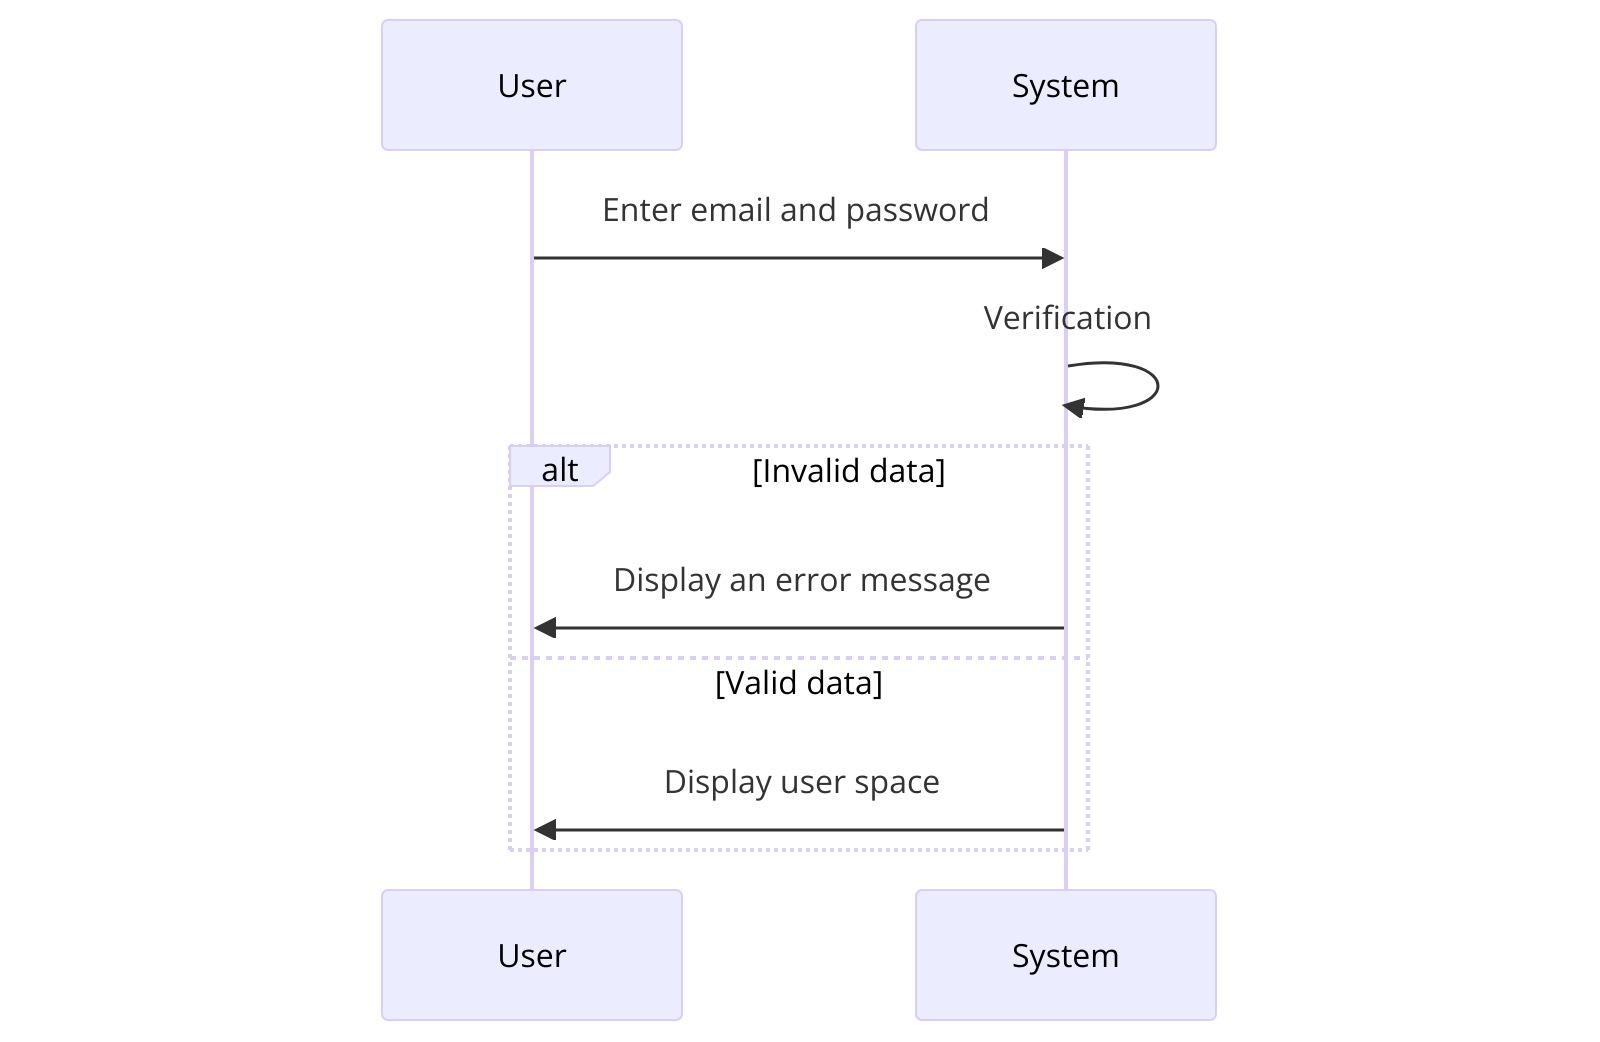
\includegraphics[width=0.8\textwidth]{images/diagram seq.png}
        \caption{the sequence diagram for the use case 'authenticate'}
        \label{fig:the sequence diagram for the use case 'authenticate'}
  \end{figure}






   
    \newpage
    Each user who wants to authenticate must access the authentication page. Then, they enter their email and password. The system validates and verifies their existence. If these credentials are valid, a message indicating that the user must activate their account via email is sent. The user then checks their email inbox and clicks on the received link to securely access their personal space. Otherwise, an error message is displayed indicating that the entered data is invalid.

